% Options for packages loaded elsewhere
\PassOptionsToPackage{unicode}{hyperref}
\PassOptionsToPackage{hyphens}{url}
%
\documentclass[
]{article}
\usepackage{amsmath,amssymb}
\usepackage{lmodern}
\usepackage{iftex}
\ifPDFTeX
  \usepackage[T1]{fontenc}
  \usepackage[utf8]{inputenc}
  \usepackage{textcomp} % provide euro and other symbols
\else % if luatex or xetex
  \usepackage{unicode-math}
  \defaultfontfeatures{Scale=MatchLowercase}
  \defaultfontfeatures[\rmfamily]{Ligatures=TeX,Scale=1}
\fi
% Use upquote if available, for straight quotes in verbatim environments
\IfFileExists{upquote.sty}{\usepackage{upquote}}{}
\IfFileExists{microtype.sty}{% use microtype if available
  \usepackage[]{microtype}
  \UseMicrotypeSet[protrusion]{basicmath} % disable protrusion for tt fonts
}{}
\makeatletter
\@ifundefined{KOMAClassName}{% if non-KOMA class
  \IfFileExists{parskip.sty}{%
    \usepackage{parskip}
  }{% else
    \setlength{\parindent}{0pt}
    \setlength{\parskip}{6pt plus 2pt minus 1pt}}
}{% if KOMA class
  \KOMAoptions{parskip=half}}
\makeatother
\usepackage{xcolor}
\IfFileExists{xurl.sty}{\usepackage{xurl}}{} % add URL line breaks if available
\IfFileExists{bookmark.sty}{\usepackage{bookmark}}{\usepackage{hyperref}}
\hypersetup{
  hidelinks,
  pdfcreator={LaTeX via pandoc}}
\urlstyle{same} % disable monospaced font for URLs
\usepackage{longtable,booktabs,array}
\usepackage{calc} % for calculating minipage widths
% Correct order of tables after \paragraph or \subparagraph
\usepackage{etoolbox}
\makeatletter
\patchcmd\longtable{\par}{\if@noskipsec\mbox{}\fi\par}{}{}
\makeatother
% Allow footnotes in longtable head/foot
\IfFileExists{footnotehyper.sty}{\usepackage{footnotehyper}}{\usepackage{footnote}}
\makesavenoteenv{longtable}
\usepackage{graphicx}
\makeatletter
\def\maxwidth{\ifdim\Gin@nat@width>\linewidth\linewidth\else\Gin@nat@width\fi}
\def\maxheight{\ifdim\Gin@nat@height>\textheight\textheight\else\Gin@nat@height\fi}
\makeatother
% Scale images if necessary, so that they will not overflow the page
% margins by default, and it is still possible to overwrite the defaults
% using explicit options in \includegraphics[width, height, ...]{}
\setkeys{Gin}{width=\maxwidth,height=\maxheight,keepaspectratio}
% Set default figure placement to htbp
\makeatletter
\def\fps@figure{htbp}
\makeatother
\setlength{\emergencystretch}{3em} % prevent overfull lines
\providecommand{\tightlist}{%
  \setlength{\itemsep}{0pt}\setlength{\parskip}{0pt}}
\setcounter{secnumdepth}{-\maxdimen} % remove section numbering
\ifLuaTeX
  \usepackage{selnolig}  % disable illegal ligatures
\fi

\author{}
\date{}

\begin{document}

\begin{longtable}[]{@{}l@{}}
\toprule
\textbf{pr 5.} A white piece of chalk is thrown onto a black horizontal
board moving at constant velocity. Initially, the chalk's \\
\midrule
\endhead
velocity was perpendicular to the board's direction of motion. \\
What is the shape of the chalk's trace on the board? \\
\bottomrule
\end{longtable}

\begin{longtable}[]{@{}l@{}}
\toprule
\endhead
 \\
\bottomrule
\end{longtable}

\begin{quote}
To solve the next problem, in addition to the previous idea we also need
to use 2, which can be rephrased in a slightly more general (but less
specific) way: some minima and maxima can be found without taking any
derivatives, in fact the solution without a derivative can turn out to
be much simpler. For this problem, an even more narrowed down
formulation would be the following.

\textbf{idea 8:} If one of two vectors is constant and the direction of
the other is fixed then the modulus of their sum is minimal if they form
a right-angled triangle.
\end{quote}

\begin{longtable}[]{@{}l@{}}
\toprule
\textbf{pr 6.} A block is pushed onto a conveyor belt. The belt is
moving at velocity \emph{v}0 = 1 m\emph{/}s, the block's initial
velocity \emph{u}0 = 2 m\emph{/}s is perpendicular to the belt's
velocity. During its subsequent motion, what is the minimum velocity of
the block \\
\midrule
\endhead
with respect to the ground? The coefficient of friction is large \\
enough to prevent the block from falling off the belt. \\
\bottomrule
\end{longtable}

\begin{longtable}[]{@{}l@{}}
\toprule
\endhead
 \\
\bottomrule
\end{longtable}

\begin{quote}
The next problem is slightly unusual, specific comments will be given
after the problem. To tackle such situation one can give seemingly
trivial but very often an overlooked advice.

\textbf{idea 9:} Read carefully the problem text, try to understand the
meaning of every statement, don't make hasty assumptions by yourself.
\end{quote}

For a well-written problem, there are no redundant sentences. Things
become more troublesome if that is not the case. Sometimes the problem
author wants to educate you more than just by giving you the very
problem, and tells you many things (such as historical background) which
are definitely interesting but unrelated to the solution of the problem.
It is OK if you are solving the problem as an exercise at home and you
have plenty of time. However, you need to develop skills of parsing fast
through such paragraphs at competitions under time pressure: you need to
make sure that there are really no important hints hidden inside.

\begin{longtable}[]{@{}l@{}}
\toprule
\textbf{pr 7.} After being kicked by a footballer, a ball started to fly
straight towards the goal at velocity \emph{v} = 25 m\emph{/}s making \\
\midrule
\endhead
an angle \emph{α} = arccos 0\emph{.}8 with the horizontal. Due to side
wind \\
blowing at \emph{u} = 10 m\emph{/}s perpendicular the initial velocity
of the \\
ball, the ball had deviated from its initial course by \emph{s} = 2 m
by \\
the time it reached the plane of the goal. Find the time that \\
it took the ball to reach the plane of the goal, if the goal was \\
situated at distance \emph{L} = 32 m from the footballer. \\
A typical problem gives all the parameter values describing a \\
system and then asks about its behaviour. Here, the system \\
might seem to be over-described: why do we need the value of
\emph{s}, \\
couldn't we just use the initial velocity to determine the flight \\
time to deduce \emph{t} = \emph{v} cos \emph{α}? Such a question might
arise, first of all, because you are used to ignoring air friction.
However, \\
no-one mentioned that you can neglect it here! Furthermore, it \\
is even evident that the air drag cannot be neglected, because \\
otherwise the ball would not depart from its free-fall trajectory! \\
\bottomrule
\end{longtable}

\begin{longtable}[]{@{}l@{}}
\toprule
\endhead
 \\
\bottomrule
\end{longtable}

\begin{quote}
2. VELOCITIES\\
It would be a very difficult task (requiring a numerical integration of a
differential equation) to estimate the trajectory of the ball subject to
a turbulent air drag. However, this is not what you need to do, because
the air drag is not described by a formula for the drag force, but
instead, by the final departure from the corresponding
free-fall-trajectory.

So, with the help of idea 9 we conclude that the air drag cannot be
neglected here. Once we have understood that, it becomes evident that we
need to apply the idea 7. However, even when equipped with this
knowledge, you might run into mathematical difficulties as there is no
direct way of expressing the flight time \emph{t} in terms of the given
quantities. Instead, you are advised to write down an equation
containing \emph{t} as an unknown, and then to solve it.

\textbf{idea 10:} It is often useful first to write down an equation (or
a system of equations) containing the required quantity as an unknown,
instead of trying to express it directly (sometimes it is necessary to
include additional unknowns that later get eliminated).

Furthermore, unlike the problems we had thus far, this problem deals
with a 3-dimensional geometry, which makes it difficult to draw sketches
on a 2-dimensional sheet of paper. Thus we need one more simple idea.

\textbf{idea 11:} It is difficult to analyse three-dimensional motion as a
whole, so whenever possible, it should be reduced to two dimensions
(projecting on a plane, looking at planes of intersection).

The next problem illustrates

\textbf{idea 12:} An elastic collision is analysed most conveniently in
the centre of mass frame of the process.

Let us derive from this idea a ready-to-use recipe when a ball collides
with a moving wall. First, since the wall is heavy, the system's centre
of mass coincides with that of the wall, hence we'll use the wall's
frame. In the frame of the centre of mass, if the collision is elastic
and there is no friction then due to the energy and momentum
conservation, the bodies will depart with the same speed as they
approached, i.e. the normal component of the ball's velocity is
reversed. If we apply the addition of velocities twice (when we move to
the wall's frame, and when we switch back to the lab frame), we arrive
at the following conclusion.

\textbf{idea 13:} For an elastic bouncing of a ball from a wall which
moves with a velocity \emph{⃗u} in the direction of the surface normal,
the normal component \emph{⃗vn} of the ball's velocity \emph{⃗v} is
increased by 2\emph{⃗u}, i.e. \emph{⃗v′n}=\emph{~−⃗vn}+ 2\emph{⃗u}.

For this problem we must also remember

\textbf{fact 1:} Angle between velocity vectors depends on the frame of
reference!
\end{quote}

\begin{longtable}[]{@{}
  >{\raggedright\arraybackslash}p{(\columnwidth - 0\tabcolsep) * \real{1.00}}@{}}
\toprule
\begin{minipage}[b]{\linewidth}\raggedright
\begin{quote}
\textbf{pr 8.} A tennis ball falls at velocity \emph{v} onto a heavy
racket and bounces back elastically. What does the racket's velocity
\end{quote}
\end{minipage} \\
\midrule
\endhead
\emph{u} have to be to make the ball bounce back at a right angle to \\
its initial trajectory and not start spinning if it did not spin \\
before the bounce? What is the angle \emph{β} between \emph{⃗u} and
the \\
normal of the racket's plane, if the corresponding angle for \emph{⃗v}
is \\
\bottomrule
\end{longtable}

\begin{longtable}[]{@{}l@{}}
\toprule
\endhead
 \\
\bottomrule
\end{longtable}

--- page 3 ---

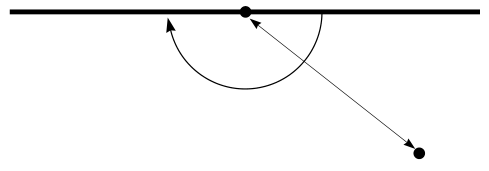
\includegraphics[width=2.26389in,height=0.79167in]{7c2ba21d717249b59a8d5c87a07c8bb7/media/image1.png}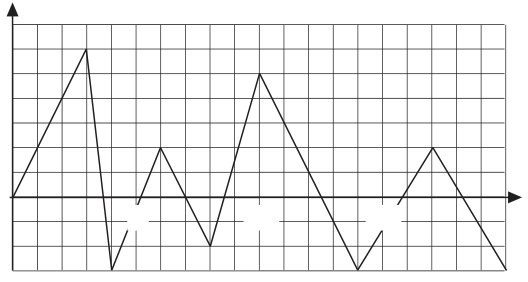
\includegraphics[width=2.44444in,height=1.30556in]{7c2ba21d717249b59a8d5c87a07c8bb7/media/image2.png}

\begin{longtable}[]{@{}
  >{\raggedright\arraybackslash}p{(\columnwidth - 10\tabcolsep) * \real{0.17}}
  >{\raggedright\arraybackslash}p{(\columnwidth - 10\tabcolsep) * \real{0.17}}
  >{\raggedright\arraybackslash}p{(\columnwidth - 10\tabcolsep) * \real{0.17}}
  >{\raggedright\arraybackslash}p{(\columnwidth - 10\tabcolsep) * \real{0.17}}
  >{\raggedright\arraybackslash}p{(\columnwidth - 10\tabcolsep) * \real{0.17}}
  >{\raggedright\arraybackslash}p{(\columnwidth - 10\tabcolsep) * \real{0.17}}@{}}
\toprule
3. ACCELERATIONS, DISPLACEMENTS & & & & & \\
\midrule
\endhead
\begin{minipage}[t]{\linewidth}\raggedright
\begin{quote}
\emph{α}?
\end{quote}
\end{minipage} & axis, the direction being given by the screw rule (if
the screw is & & & & \\
\begin{minipage}[t]{\linewidth}\raggedright
\begin{quote}
If we keep in mind the idea 9 and read the text carefully, we notice
that the racket is \emph{heavy} so that we can use the idea 13.
\end{quote}
\end{minipage} & rotated in the same way as the body, the vector points
in the direction of the screw movement). & & & & \\
\begin{minipage}[t]{\linewidth}\raggedright
Also, pay attention that the ball will not rotate after the collision
--- this is important for finding the parallel (to the racket's plane)
component of the velocity.

\begin{quote}
Earlier we mentioned that vectors can be dealt with either geometrically
(e.g. by applying the triangle rule for a sum of vectors and solving a
trigonometrical problem), or algebraically using projections. Quite
often, geometrical approach provides shorter solutions, but not always;
this observation leads us to
\end{quote}
\end{minipage} & \textbf{idea 17:} When switching between rotating
frames of reference, angular velocities are to be added in the same as
transla & & & & \\
& tional velocities in the case of translationally moving frames of & &
& & \\
& reference. NB! This remains valid even if the angular velocit & & &
& \\
& ies are not parallel (although non-small rotation angles can be & & &
& \\
& added only as long as the rotation axis remains unchanged). & & & & \\
& This idea is illustrated by a relatively simple problem below. & & &
& \\
\begin{minipage}[t]{\linewidth}\raggedright
\begin{quote}
the following recommendation.

\textbf{idea 14:} For vectorial calculations, prefer geometrical
approach, but if it seems unreasonable (e.g. some of the conditions
\end{quote}
\end{minipage} & \textbf{pr 9.} Vertical mirror with two reflecting
surfaces (front and back) rotates around a vertical axis as shown in
figure, with & & & & \\
& angular speed \emph{ω}. There is an unmoving point source of light
\emph{S} & & & & \\
\begin{minipage}[t]{\linewidth}\raggedright
\begin{quote}
are formulated through the projections of the vectors) switch
\end{quote}
\end{minipage} & at a distance \emph{a} from the rotation axis. Find the
speed of the & & & & \\
\begin{minipage}[t]{\linewidth}\raggedright
\begin{quote}
to the algebraic approach and write expressions down in terms
\end{quote}
\end{minipage} & image of the point source as a function of time. & & &
& \\
\begin{minipage}[t]{\linewidth}\raggedright
\begin{quote}
of components.
\end{quote}
\end{minipage} & ω & & & & \\
\begin{minipage}[t]{\linewidth}\raggedright
\begin{quote}
For the algebraic approach, \textbf{optimal choice of axes} is very
\end{quote}
\end{minipage} & a & & & & \\
\begin{minipage}[t]{\linewidth}\raggedright
\begin{quote}
important. ``Optimal'' means that the conditions are written in the
simplest possible way. Sometimes it may happen that
\end{quote}
\end{minipage} & S & & & & \\
\begin{minipage}[t]{\linewidth}\raggedright
\begin{quote}
the most useful coordinate axes are not even at right angles.
\end{quote}
\end{minipage} & & & & & \\
\begin{minipage}[t]{\linewidth}\raggedright
\begin{quote}
For the problem 8, geometrical solution turns out to be simpler, but
more difficult to come up with. This is quite typical: algebraic approach
leads to a brute-force-solution when it is clear from the beginning what
you need to do, but the calculations are mathematically long. Still,
there are no fundamental
\end{quote}
\end{minipage} & \textbf{3} &
\begin{minipage}[t]{\linewidth}\raggedright
\begin{quote}
\textbf{ACCELERATIONS, DISPLACEMENTS}
\end{quote}
\end{minipage} & & & \\
& Thus far we dealt with instantaneous or constant velocities, and & & &
& \\
& in few cases we applied a simple formula \emph{s} = \emph{vt} for
displace & & & & \\
& ments. In general, when the velocity \emph{⃗v} is not constant, the
dis & & & & \\
difficulties and you just need to execute it. &
\begin{minipage}[t]{\linewidth}\raggedright
\begin{quote}
As long as the
\end{quote}
\end{minipage} & placement is found as the curve under the graph of the
velocity & & & \\
\begin{minipage}[t]{\linewidth}\raggedright
\begin{quote}
mathematical part will not be \emph{unreasonably long} or leading to
fundamental difficulties (such as unsolvable equations), brute force
approach is still OK: figuring out an elegant solution can also take some
time.

Typically, the geometrical solutions of physics problems rep
\end{quote}
\end{minipage} & as a function of time. & For instance, the displacement
along & & & \\
& \emph{x}-coordinate ∆\emph{x} is surface area under the graph
\emph{vx} = \emph{vx}(\emph{t}); mathematically we can write it via
integral ∆\emph{x} =∫\emph{vx}(\emph{t})\emph{dt}. You don't need to
know more about integrals right now, just that it represents surface
areas under graphs. & & & & \\
\begin{minipage}[t]{\linewidth}\raggedright
\begin{quote}
resent very simple geometrical tasks and hence, finding these
\end{quote}
\end{minipage} & \textbf{idea 18:} Calculation of many physical
quantities can be reduced (sometimes not in an obvious way) to the
calculation of & & & & \\
\begin{minipage}[t]{\linewidth}\raggedright
\begin{quote}
shorter-than-algebraic solutions is also quite easy. In this case,
\end{quote}
\end{minipage} & & & & & \\
\begin{minipage}[t]{\linewidth}\raggedright
\begin{quote}
however, the geometrical task turns out to be quite a tricky
\end{quote}
\end{minipage} & & & & & \\
& surface areas under a graph (i.e. to an integral). In particular: & &
& & \\
problem. & \begin{minipage}[t]{\linewidth}\raggedright
\begin{quote}
While the idea 14 suggests that the algebraic ap
\end{quote}
\end{minipage} & & & & \\
& & distance is the area under a \emph{v−t} curve (velocity-time),
velocity the area below an \emph{a~− t} curve etc. & & & \\
\begin{minipage}[t]{\linewidth}\raggedright
\begin{quote}
proach is good for problem 8 (the no-rotation-requirement gives
\end{quote}
\end{minipage} & & & & & \\
\begin{minipage}[t]{\linewidth}\raggedright
\begin{quote}
us a condition for the parallel component of the velocity), it is
\end{quote}
\end{minipage} & & & & & \\
\begin{minipage}[t]{\linewidth}\raggedright
\begin{quote}
recommended that you try both methods here. In both cases
\end{quote}
\end{minipage} & Note that drawing a graph is not always absolutely
necessary (if & & & & \\
\begin{minipage}[t]{\linewidth}\raggedright
\begin{quote}
you need one more mathematical idea.
\end{quote}
\end{minipage} & you are skilled with integrals, formulae can be derived
analytic & & & & \\
\begin{minipage}[t]{\linewidth}\raggedright
\begin{quote}
\textbf{idea 15:} Two vectors \emph{⃗a} = (\emph{ax, ay, az})
and\emph{⃗b} = (\emph{bx, by, bz}) are perpendicular if their scalar
product is zero, \emph{axbx} + \emph{ayby} + \emph{azbz} = 0. (This
assumes that the axes \emph{x}, \emph{y} and \emph{z} are perpendicular
to each other.)
\end{quote}
\end{minipage} & ally, without drawing graphs), but doing it helps to
imagine the & & & & \\
& process. Visualisation of this kind is always beneficial, it sim & & &
& \\
& plifies finding the solution and reduces the chances of making & & &
& \\
& mistakes. & & & & \\
& \textbf{pr 10.} A particle starts from the origin of coordinates; the
figure shows its velocity as a function of time. What is its & & & & \\
\begin{minipage}[t]{\linewidth}\raggedright
\begin{quote}
\textbf{idea 16:} For trigonometric problems involving right triangles
keep in mind that the circumcentre of a right triangle is at the
\end{quote}
\end{minipage} & & & & & \\
& \begin{minipage}[t]{\linewidth}\raggedright
maximum shift from the origin?

\begin{quote}
v(m/s)
\end{quote}
\end{minipage} & & & & \\
\begin{minipage}[t]{\linewidth}\raggedright
\begin{quote}
centre of the hypotenuse, hence the median drawn from the
\end{quote}
\end{minipage} & & & & & \\
& \begin{minipage}[t]{\linewidth}\raggedright
\begin{quote}
6
\end{quote}
\end{minipage} & & & & \\
\begin{minipage}[t]{\linewidth}\raggedright
\begin{quote}
right angle divides the triangle into two isosceles triangles, and
\end{quote}
\end{minipage} & & & & & \\
\begin{minipage}[t]{\linewidth}\raggedright
\begin{quote}
the right angle into the angles equal to the acute angles of the
\end{quote}
\end{minipage} & 4 & 5 & 10 & 15 &
\begin{minipage}[t]{\linewidth}\raggedright
\begin{quote}
t(s)
\end{quote}
\end{minipage} \\
\begin{minipage}[t]{\linewidth}\raggedright
\begin{quote}
triangle.
\end{quote}
\end{minipage} & 2 & & & & \\
\begin{minipage}[t]{\linewidth}\raggedright
\begin{quote}
Idea 1 told us to make use of switching between different
\end{quote}
\end{minipage} & 0 & & & & \\
\begin{minipage}[t]{\linewidth}\raggedright
\begin{quote}
frames of reference. This idea can be also used when dealing
\end{quote}
\end{minipage} & -2 & & & & \\
with rotational motion. & & & & & \\
\begin{minipage}[t]{\linewidth}\raggedright
\begin{quote}
\textbf{def. 3:} Angular velocity \emph{⃗ω} equals by modulus to the
rotation angle (in radians) per unit time, and is parallel to the
rotation
\end{quote}
\end{minipage} & The next problem is much more difficult, although it is
also reduced to finding a surface area; due to difficulty, the full & & &
& \\
\bottomrule
\end{longtable}

\begin{longtable}[]{@{}l@{}}
\toprule
\endhead
 \\
\bottomrule
\end{longtable}

\begin{longtable}[]{@{}l@{}}
\toprule
\endhead
 \\
\bottomrule
\end{longtable}

--- page 4 ---

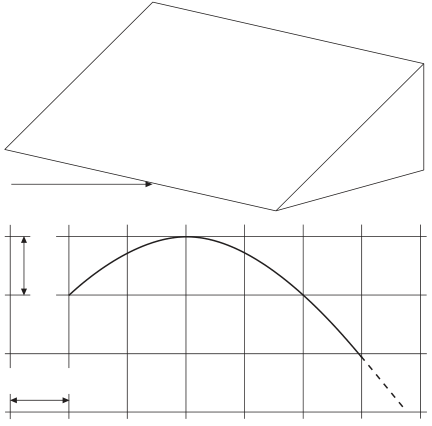
\includegraphics[width=2in,height=1.97222in]{7c2ba21d717249b59a8d5c87a07c8bb7/media/image3.png}

\begin{longtable}[]{@{}
  >{\raggedright\arraybackslash}p{(\columnwidth - 4\tabcolsep) * \real{0.33}}
  >{\raggedright\arraybackslash}p{(\columnwidth - 4\tabcolsep) * \real{0.33}}
  >{\raggedright\arraybackslash}p{(\columnwidth - 4\tabcolsep) * \real{0.33}}@{}}
\toprule
3. ACCELERATIONS, DISPLACEMENTS & & \\
\midrule
\endhead
\begin{minipage}[t]{\linewidth}\raggedright
\begin{quote}
spective perpendicular components, \emph{⃗g} = \emph{⃗gx}+\emph{⃗gy}
with \emph{gx} = sin \emph{α} and \emph{gy} = cos \emph{α}, \emph{α}
being the angle between the surface and the horizon.
\end{quote}
\end{minipage} & \begin{minipage}[t]{\linewidth}\raggedright
\begin{quote}
of the two surfaces and \emph{y}-axis lays on the inclined surface,
\emph{x}, \emph{y},
\end{quote}
\end{minipage} & \\
& \begin{minipage}[t]{\linewidth}\raggedright
\begin{quote}
and \emph{z}-motions are all separated; at the impact, \emph{vz} goes to
zero, and due to the absence of friction, \emph{vx} and \emph{vy} are
preserved. In this problem, however, the transition from one surface
\end{quote}
\end{minipage} & \\
\begin{minipage}[t]{\linewidth}\raggedright
\begin{quote}
During a collision, as there is no friction force, \emph{vx} (parallel
to the surface velocity component) does not change, i.e. it does
\end{quote}
\end{minipage} & & \\
& \begin{minipage}[t]{\linewidth}\raggedright
\begin{quote}
to the other is smooth: around the line separating the two
\end{quote}
\end{minipage} & \\
& \begin{minipage}[t]{\linewidth}\raggedright
\begin{quote}
flat surfaces, there is a narrow region where the surface has a
\end{quote}
\end{minipage} & \\
not ``notice'' that there was a collision: in order to analyse the &
& \\
& \begin{minipage}[t]{\linewidth}\raggedright
\begin{quote}
curvature. Within this narrow region, the motion in \emph{y}- and
\end{quote}
\end{minipage} & \\
evolution of the \emph{x}-coordinate, we can completely forget about &
& \\
& \begin{minipage}[t]{\linewidth}\raggedright
\begin{quote}
\emph{z}-directions cannot be separated from each other, and we need
\end{quote}
\end{minipage} & \\
\begin{minipage}[t]{\linewidth}\raggedright
\begin{quote}
the changes of the \emph{y}-coordinate (and vice versa).
\end{quote}
\end{minipage} & & \\
& \begin{minipage}[t]{\linewidth}\raggedright
\begin{quote}
one more idea.
\end{quote}
\end{minipage} & \\
\begin{minipage}[t]{\linewidth}\raggedright
\begin{quote}
If the surface is curved, generally such a separation is no
\end{quote}
\end{minipage} & & \\
& \begin{minipage}[t]{\linewidth}\raggedright
\begin{quote}
\textbf{idea 21:} If a force is perpendicular to the direction of motion
(normal force when sliding along a curved surface, tension in a
\end{quote}
\end{minipage} & \\
longer possible. Indeed, previously \emph{x} was independent of \emph{y}
be & & \\
cause the dependence of the acceleration on the coordinates is & & \\
introduced by the normal force, which is a function of \emph{y} only, &
\begin{minipage}[t]{\linewidth}\raggedright
\begin{quote}
rope when a moving body is attached to an unstretchable rope
\end{quote}
\end{minipage} & \\
and has no \emph{x}-component. &
\begin{minipage}[t]{\linewidth}\raggedright
\begin{quote}
If the surface is curved, it is im
\end{quote}
\end{minipage} & \begin{minipage}[t]{\linewidth}\raggedright
\begin{quote}
fixed at the other end, force on a charge in magnetic field) then
\end{quote}
\end{minipage} \\
possible to have the \emph{x}-axis to be everywhere parallel to the &
\begin{minipage}[t]{\linewidth}\raggedright
\begin{quote}
the velocity vector can only turn, its modulus will not change.4
\end{quote}
\end{minipage} & \\
surface: the acceleration due to the normal force has both non &
\begin{minipage}[t]{\linewidth}\raggedright
\begin{quote}
\textbf{pr 15.} Three turtles are initially situated in the corners of
an equilateral triangle at distances 1 m from one another. They
\end{quote}
\end{minipage} & \\
vanishing \emph{x} and \emph{y} components, and depends both on \emph{x}
and \emph{y} & & \\
coordinates. However, in the case of side surfaces of cylinders, & & \\
prisms and other generalized cylinders3, it is still possible to &
\begin{minipage}[t]{\linewidth}\raggedright
\begin{quote}
move at constant velocity 10 cm\emph{/}s in such a way that the first
\end{quote}
\end{minipage} & \\
find one axis \emph{x} which is everywhere parallel to the surface and &
\begin{minipage}[t]{\linewidth}\raggedright
\begin{quote}
always heading towards the second, the second towards the
\end{quote}
\end{minipage} & \\
hence, motion along \emph{x} can be separated from the motion in &
\begin{minipage}[t]{\linewidth}\raggedright
\begin{quote}
third and the third towards the first. After what time will they
\end{quote}
\end{minipage} & \\
\begin{minipage}[t]{\linewidth}\raggedright
\begin{quote}
\emph{y~− z}-plane.
\end{quote}
\end{minipage} & \begin{minipage}[t]{\linewidth}\raggedright
\begin{quote}
meet?
\end{quote}
\end{minipage} & \\
\textbf{pr 13.} & \begin{minipage}[t]{\linewidth}\raggedright
\begin{quote}
An elastic ball is released above an inclined plane
\end{quote}
\end{minipage} & Two approaches are possible here: first, we may go into
the \\
& & frame of reference rotating with the turtles, in which case we \\
(inclination angle \emph{α}) at distance \emph{d} from the plane. What
is & & \\
& apply the following idea. & \\
\begin{minipage}[t]{\linewidth}\raggedright
\begin{quote}
the distance between the first bouncing point and the second?
\end{quote}
\end{minipage} & & \\
& \textbf{idea 22:} Sometimes even a reference frame undergoing very
complex motion can be useful. & \\
\begin{minipage}[t]{\linewidth}\raggedright
\begin{quote}
Collisions occur without friction.
\end{quote}
\end{minipage} & & \\
\begin{minipage}[t]{\linewidth}\raggedright
\begin{quote}
The next problem makes also use of the idea 20; however, one
\end{quote}
\end{minipage} & & \\
& Alternatively, we can use & \\
\begin{minipage}[t]{\linewidth}\raggedright
\begin{quote}
more idea is needed, see below.
\end{quote}
\end{minipage} & & \\
\begin{minipage}[t]{\linewidth}\raggedright
\begin{quote}
\textbf{pr 14.} A puck slides onto an icy inclined plane with
inclination angle \emph{α}. The angle between the plane's edge and the
puck's initial velocity \emph{v}0 = 10 m\emph{/}s is \emph{β} =
60\emph{◦}. The trace left by the puck on the plane is given in the
figure (this is only a part of the trajectory). Find \emph{α} under the
assumption that
\end{quote}
\end{minipage} & \textbf{idea 23:} Instead of calculating physical
velocities, it is sometimes wise to look at the rate of change of some
distance, the & \\
& ratio of two lengths, etc. & \\
& The following problem requires integration5, so it can be & \\
& skipped by those who are not familiar with it. & \\
\begin{minipage}[t]{\linewidth}\raggedright
\begin{quote}
friction can be neglected and that transition onto the slope was smooth.
\end{quote}
\end{minipage} & \textbf{pr 16.} &
\begin{minipage}[t]{\linewidth}\raggedright
\begin{quote}
An ant is moving along a rubber band at velocity
\end{quote}
\end{minipage} \\
& \begin{minipage}[t]{\linewidth}\raggedright
\begin{quote}
\emph{v} = 1 cm\emph{/}s. One end of the rubber band (the one from which
\end{quote}
\end{minipage} & \\
the ant started) is fixed to a wall, the other (initially at dis & & \\
tance \emph{L} = 1 m from the wall) is pulled at \emph{u} = 1
m\emph{/}s. Will the & & \\
ant reach the other end of the band? If yes then when will it & & \\
β & α & happen? \\
& & Here we need to apply the \\
\begin{minipage}[t]{\linewidth}\raggedright
\begin{quote}
\textbf{idea 24:} For some problems, optimal choice of parametriza\\
tion can simplify mathematical calculations significantly. An
\end{quote}
\end{minipage} & & \\
\begin{minipage}[t]{\linewidth}\raggedright
\begin{quote}
2.5m
\end{quote}
\end{minipage} & incomplete list of options: Cartesian, polar,
cylindrical, and spherical coordinates; travel distance;
\emph{Lagrangian coordinates} & \\
(i.e. for fluids flow using the initial coordinate of a fluid particle &
& \\
\begin{minipage}[t]{\linewidth}\raggedright
\begin{quote}
The last sentence here is very important: if the transition is
\emph{sharp}, the puck approaches the inclined plane by sliding along
\end{quote}
\end{minipage} & instead of its current coordinate); relative position
of a particle according to a certain ranking scheme, etc. & \\
\begin{minipage}[t]{\linewidth}\raggedright
\begin{quote}
the horizontal and collides with it --- either elastically in which
\end{quote}
\end{minipage} & Here, the problem itself contains a hint about which
type of & \\
\begin{minipage}[t]{\linewidth}\raggedright
\begin{quote}
case it jumps up, or plastically. In particular, if the collision
\end{quote}
\end{minipage} & parametrization is to be used. It is clear that the
Cartesian & \\
\begin{minipage}[t]{\linewidth}\raggedright
\begin{quote}
is perfectly plastic then that part of the kinetic energy which
\end{quote}
\end{minipage} & coordinate of the ant is not good: it does not reflect
the pro & \\
\begin{minipage}[t]{\linewidth}\raggedright
\begin{quote}
is associated with the motion along the surface normal of the
\end{quote}
\end{minipage} & gress of the ant in advancing along the rubber band. In
order & \\
\begin{minipage}[t]{\linewidth}\raggedright
\begin{quote}
inclined plane is lost. More specifically, if we introduce perpen
\end{quote}
\end{minipage} & to describe such a progress, we can use the relative
position on & \\
\begin{minipage}[t]{\linewidth}\raggedright
\begin{quote}
dicular coordinates so that the \emph{x}-axis is along the contact line
\end{quote}
\end{minipage} & the band: which fraction \emph{k} of the rubber is left
behind; the ant & \\
\bottomrule
\end{longtable}

\begin{longtable}[]{@{}l@{}}
\toprule
\endhead
 \\
\bottomrule
\end{longtable}

\begin{longtable}[]{@{}l@{}}
\toprule
\endhead
 \\
\bottomrule
\end{longtable}

\begin{longtable}[]{@{}l@{}}
\toprule
\endhead
 \\
\bottomrule
\end{longtable}

\begin{longtable}[]{@{}
  >{\raggedright\arraybackslash}p{(\columnwidth - 0\tabcolsep) * \real{1.00}}@{}}
\toprule
 \\
\midrule
\endhead
\begin{minipage}[t]{\linewidth}\raggedright
\begin{quote}
3Surfaces with constant cross-sections.

4This is the energy conservation law using the fact that forces
perpendicular to the velocity will not perform work.

5You may find helpful to know that∫\emph{ax}+\emph{b}= \emph{a−}1
ln(\emph{ax} + \emph{b}) + \emph{C}--- page 6 ---
\end{quote}
\end{minipage} \\
\bottomrule
\end{longtable}

\begin{longtable}[]{@{}l@{}}
\toprule
\endhead
 \\
\bottomrule
\end{longtable}

\begin{longtable}[]{@{}l@{}}
\toprule
time will the string be fully wound around the cylinder again, \\
\midrule
\endhead
this time the other way round? {[}This problem leads to a very \\
simple differential equation; if you don't know how to solve it, the
following equality can be helpful: \emph{ldldt}=
1\emph{d}(\emph{l}2)\emph{dt}.{]} \\
\bottomrule
\end{longtable}

v

r

\begin{longtable}[]{@{}l@{}}
\toprule
\textbf{pr 47.} A heavy box is being pulled using two tractors. One of
these has velocity \emph{v}1, the other \emph{v}2, the angle between
velocities is \emph{α}. What is the velocity of the box, if we assume
that \\
\midrule
\endhead
the ropes are parallel to velocity vectors? \\
\bottomrule
\end{longtable}

\begin{longtable}[]{@{}l@{}}
\toprule
\endhead
 \\
\bottomrule
\end{longtable}

v2

v1

α

\begin{longtable}[]{@{}
  >{\raggedright\arraybackslash}p{(\columnwidth - 0\tabcolsep) * \real{1.00}}@{}}
\toprule
\begin{minipage}[b]{\linewidth}\raggedright
\begin{quote}
\textbf{pr 48.} A boy is running on a large field of ice with velocity
\emph{v} = 5 m\emph{/}s toward the north. The coefficient of friction
between
\end{quote}
\end{minipage} \\
\midrule
\endhead
his feet and the ice is \emph{µ} = 0\emph{.}1. Assume as a simplification
that \\
the reaction force between the boy and the ice stays constant \\
(in reality it varies with every push, but the assumption is jus \\
tified by the fact that the value averaged over one step stays \\
\begin{minipage}[t]{\linewidth}\raggedright
\begin{quote}
constant).
\end{quote}
\end{minipage} \\
\textbf{i)} What is the minimum time necessary for him to change his \\
moving direction to point towards the east so that the final \\
\begin{minipage}[t]{\linewidth}\raggedright
\begin{quote}
speed is also \emph{v} = 5 m\emph{/}s?
\end{quote}
\end{minipage} \\
\begin{minipage}[t]{\linewidth}\raggedright
\begin{quote}
\textbf{i)} What is the shape of the optimal trajectory called?
\end{quote}
\end{minipage} \\
\begin{minipage}[t]{\linewidth}\raggedright
\begin{quote}
\textbf{pr 49.} A ball thrown with an initial speed \emph{v}0 moves in a
homogeneous gravitational field of strength \emph{g}; neglect the air
\end{quote}
\end{minipage} \\
drag. The throwing point can be freely selected on the ground \\
level \emph{z} = 0, and the launching angle can be adjusted as
needed; \\
the aim is to hit the topmost point of a spherical building of \\
radius \emph{R} (see fig.) with as small as possible initial speed
\emph{v}0 (prior hitting the target, bouncing off the roof is not
allowed). \\
Sketch qualitatively the shape of the optimal trajectory of the \\
\begin{minipage}[t]{\linewidth}\raggedright
\begin{quote}
ball. What is the minimal launching speed \emph{v}min needed to hit the
topmost point of a spherical building of radius \emph{R}?
\end{quote}
\end{minipage} \\
\bottomrule
\end{longtable}

\begin{longtable}[]{@{}l@{}}
\toprule
\endhead
 \\
\bottomrule
\end{longtable}

\begin{longtable}[]{@{}l@{}}
\toprule
\endhead
 \\
\bottomrule
\end{longtable}

z

\begin{longtable}[]{@{}
  >{\raggedright\arraybackslash}p{(\columnwidth - 2\tabcolsep) * \real{0.50}}
  >{\raggedright\arraybackslash}p{(\columnwidth - 2\tabcolsep) * \real{0.50}}@{}}
\toprule
\begin{minipage}[b]{\linewidth}\raggedright
\begin{quote}
7. CONCLUSION
\end{quote}
\end{minipage} & \\
\midrule
\endhead
axis was vertical, and the disk slid and rotated freely on a ho & \\
rizontal smooth ice surface. What was the speed of the centre & \\
of the disk? You can take measurements from the figure using & \\
\begin{minipage}[t]{\linewidth}\raggedright
\begin{quote}
a ruler.
\end{quote}
\end{minipage} & \begin{minipage}[t]{\linewidth}\raggedright
\begin{quote}
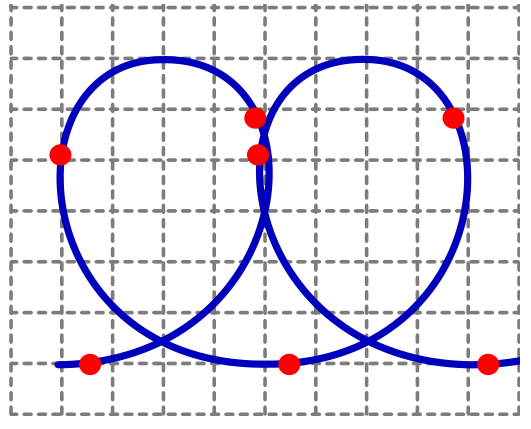
\includegraphics[width=2.45833in,height=1.98611in]{7c2ba21d717249b59a8d5c87a07c8bb7/media/image4.png}
\end{quote}
\end{minipage} \\
\begin{minipage}[t]{\linewidth}\raggedright
\begin{quote}
\textbf{pr 51.} There is a capital \emph{O} and three cities \emph{A},
\emph{B} and \emph{C}, connected with the capital via roads 1, 2, and 3
as shown in the left
\end{quote}
\end{minipage} & \\
figure. Each road has length 2\emph{a}. Two cars travel from one city
& \\
to another: they depart from their respective starting points & \\
simultaneously, and travel with a constant speed \emph{v}. The figure
& \\
on the right depicts the increasing rate of the distance between & \\
the cars (negative values means that the distance decreases) as & \\
measured by the GPS devices of the cars. The turns are taken & \\
by the cars so fast that the GPS devices will not record the & \\
\begin{minipage}[t]{\linewidth}\raggedright
\begin{quote}
behaviour during these periods.
\end{quote}
\end{minipage} & \\
\textbf{i)} Which cities were the starting and destination points of the
& \\
\begin{minipage}[t]{\linewidth}\raggedright
\begin{quote}
cars? Motivate your answer.
\end{quote}
\end{minipage} & \\
\begin{minipage}[t]{\linewidth}\raggedright
\begin{quote}
\textbf{ii)} What is the surface area between the \emph{v}dist -graph
and the \emph{t}-axis for the interval from \emph{t} = 0 to \emph{t} =
\emph{a/v}?
\end{quote}
\end{minipage} & \\
\textbf{iii)} Now let us consider a case when three cars (denoted by
\emph{A}, & \\
\emph{B}, and \emph{C}) depart simultaneously from their cities
(\emph{A}, \emph{B}, and & \\
\emph{C}, respectively) towards the capital; all the cars travel with a
& \\
constant speed \emph{v}. Sketch the graphs for the distance changing
& \\
rate for the following car pairs: \emph{A~− B} and \emph{B~− C}.
\textbf{iv)} Suppose that now the GPS-devices are good enough to re & \\
cord the periods of taking the turns. Sketch a new appropriate & \\
\begin{minipage}[t]{\linewidth}\raggedright
\begin{quote}
graph for the pair of cars \emph{B~− C}. The curvature of the turns is
small enough so that the cars can still keep theirs speed \emph{v}.A B
vdist
\end{quote}
\end{minipage} & \\
\bottomrule
\end{longtable}

\begin{longtable}[]{@{}l@{}}
\toprule
\endhead
 \\
\bottomrule
\end{longtable}

\begin{quote}
road 1
\end{quote}

\begin{longtable}[]{@{}
  >{\raggedright\arraybackslash}p{(\columnwidth - 2\tabcolsep) * \real{0.50}}
  >{\raggedright\arraybackslash}p{(\columnwidth - 2\tabcolsep) * \real{0.50}}@{}}
\toprule
\endhead
\begin{minipage}[t]{\linewidth}\raggedright
\begin{quote}
a
\end{quote}
\end{minipage} & a \\
\bottomrule
\end{longtable}

road 2

\begin{longtable}[]{@{}
  >{\raggedright\arraybackslash}p{(\columnwidth - 14\tabcolsep) * \real{0.12}}
  >{\raggedright\arraybackslash}p{(\columnwidth - 14\tabcolsep) * \real{0.12}}
  >{\raggedright\arraybackslash}p{(\columnwidth - 14\tabcolsep) * \real{0.12}}
  >{\raggedright\arraybackslash}p{(\columnwidth - 14\tabcolsep) * \real{0.12}}
  >{\raggedright\arraybackslash}p{(\columnwidth - 14\tabcolsep) * \real{0.12}}
  >{\raggedright\arraybackslash}p{(\columnwidth - 14\tabcolsep) * \real{0.12}}
  >{\raggedright\arraybackslash}p{(\columnwidth - 14\tabcolsep) * \real{0.12}}
  >{\raggedright\arraybackslash}p{(\columnwidth - 14\tabcolsep) * \real{0.12}}@{}}
\toprule
\begin{minipage}[b]{\linewidth}\raggedright
\begin{quote}
90o
\end{quote}
\end{minipage} & a & O & a & 90o &
\begin{minipage}[b]{\linewidth}\raggedright
\begin{quote}
0
\end{quote}
\end{minipage} & av & 2av t \\
\midrule
\endhead
& & \begin{minipage}[t]{\linewidth}\raggedright
\begin{quote}
90o
\end{quote}
\end{minipage} & & & & & \\
\bottomrule
\end{longtable}

\begin{longtable}[]{@{}
  >{\raggedright\arraybackslash}p{(\columnwidth - 10\tabcolsep) * \real{0.17}}
  >{\raggedright\arraybackslash}p{(\columnwidth - 10\tabcolsep) * \real{0.17}}
  >{\raggedright\arraybackslash}p{(\columnwidth - 10\tabcolsep) * \real{0.17}}
  >{\raggedright\arraybackslash}p{(\columnwidth - 10\tabcolsep) * \real{0.17}}
  >{\raggedright\arraybackslash}p{(\columnwidth - 10\tabcolsep) * \real{0.17}}
  >{\raggedright\arraybackslash}p{(\columnwidth - 10\tabcolsep) * \real{0.17}}@{}}
\toprule
C & road 3 & \begin{minipage}[b]{\linewidth}\raggedright
\begin{quote}
a
\end{quote}
\end{minipage} & - & \begin{minipage}[b]{\linewidth}\raggedright
\begin{quote}
v0
\end{quote}
\end{minipage} & \\
\midrule
\endhead
& a & 90o & & - 0v & \begin{minipage}[t]{\linewidth}\raggedright
\begin{quote}
2
\end{quote}
\end{minipage} \\
\bottomrule
\end{longtable}

x

\begin{longtable}[]{@{}
  >{\raggedright\arraybackslash}p{(\columnwidth - 0\tabcolsep) * \real{1.00}}@{}}
\toprule
\begin{minipage}[b]{\linewidth}\raggedright
\begin{quote}
\textbf{pr 50.} The figure represents a photo which was taken using a
very long exposure time (camera was pointing directly down).
\end{quote}
\end{minipage} \\
\midrule
\endhead
What you can see is a trace of a blue lamp which burned con \\
tinuously, but also flashed periodically with a red light (after \\
each \emph{t} = 0\emph{.}1 s. The lamp was fixed to the surface of a
solid \\
disk, at the distance \emph{a} = 4\emph{.}5 cm from its symmetry axis.
The \\
\bottomrule
\end{longtable}

\begin{longtable}[]{@{}l@{}}
\toprule
\endhead
 \\
\bottomrule
\end{longtable}

\begin{longtable}[]{@{}
  >{\raggedright\arraybackslash}p{(\columnwidth - 0\tabcolsep) * \real{1.00}}@{}}
\toprule
\begin{minipage}[b]{\linewidth}\raggedright
\begin{quote}
\textbf{pr 52.} Consider two rings with radius \emph{r} as depicted in
the figure: the blue ring is at rest, and the yellow ring rotates
\end{quote}
\end{minipage} \\
\midrule
\endhead
around the point \emph{O} (which is one of the intersection points \\
of the two rings) with a constant angular speed \emph{ω}. Find the \\
\begin{minipage}[t]{\linewidth}\raggedright
\begin{quote}
minimal and maximal speeds \emph{v}min and \emph{v}max of the other
intersection point of the two rings.
\end{quote}
\end{minipage} \\
\bottomrule
\end{longtable}

\begin{longtable}[]{@{}l@{}}
\toprule
\endhead
 \\
\bottomrule
\end{longtable}

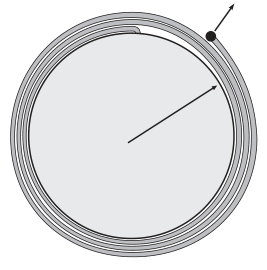
\includegraphics[width=1.23611in,height=1.25in]{7c2ba21d717249b59a8d5c87a07c8bb7/media/image5.png}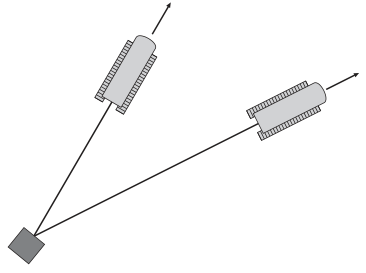
\includegraphics[width=1.69444in,height=1.26389in]{7c2ba21d717249b59a8d5c87a07c8bb7/media/image6.png}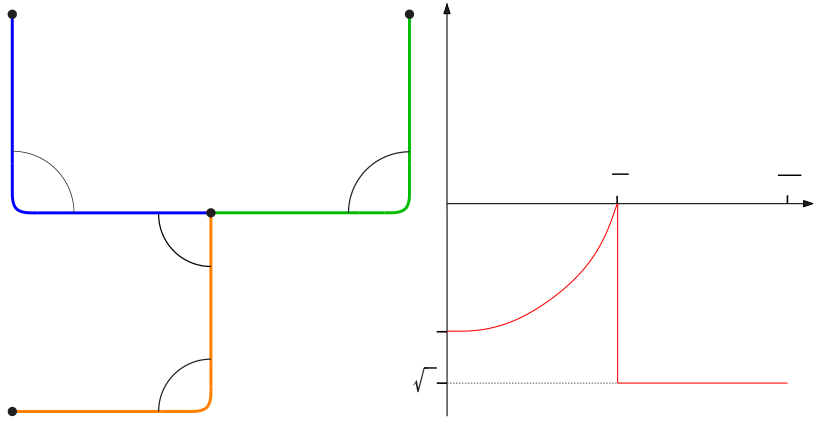
\includegraphics[width=3.79167in,height=1.98611in]{7c2ba21d717249b59a8d5c87a07c8bb7/media/image7.png}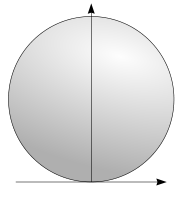
\includegraphics[width=0.84722in,height=0.91667in]{7c2ba21d717249b59a8d5c87a07c8bb7/media/image8.png}

--- page 16 ---

\end{document}
